%%%%%%%%%%%%%%%%%%%%%%%%%%%%%%%%%%%%%
\section{Methods}
\label{sec:Methods}

For convince a subversion repository was created to manage the developed code base, and all source code is available by anonymous checkout from \verb+http://www.murphs-code-repository.googlecode.com/svn/trunk/layeredPolymerTracking+. Revision 360 was the code base used to generate the results shown in \ref{sec:Results}.

\subsubsection{Detector Geometry}
The geometry was setup such that it is possible to define multiple layers of detectors, as shown in Figure \ref{fig:LayerDetectorGeo}.
This was done by creating a 
\begin{figure} 
    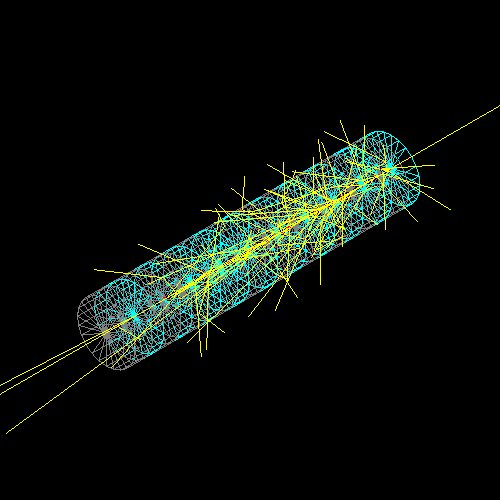
\includegraphics[width=\figurewidth]{10LayerGamma}
	\caption{10 Layer Detector with a simulated gamma event}
    \label{fig:LayerDetectorGeo}
\end{figure}
\subsubsection{Physics Lists}
